\section{Pendahuluan}
\subsection{Latar Belakang}
Praktikum ini meliputi Crimping dan Routing IPv4, yang merupakan dasar dalam pengelolaan jaringan komputer yang sangat penting untuk memastikan konektivitas yang stabil dan efektif antara perangkat-perangkat dalam jaringan. Crimping adalah proses memasang konektor RJ45 pada kabel UTP, yang digunakan untuk menghubungkan perangkat-perangkat seperti komputer, printer, atau router dalam jaringan lokal. Teknik ini sangat penting karena pengkabelan yang benar dan terstruktur memastikan data dapat dikirimkan dengan efisien dan tanpa gangguan. Sedangkan routing IPv4 adalah proses mengatur jalur yang akan dilalui oleh data dalam jaringan dengan menggunakan router.
Terdapat dua jenis routing yang umum digunakan: routing statis, di mana administrator menentukan jalur secara manual, dan routing dinamis, yang memungkinkan router saling bertukar informasi untuk menentukan jalur terbaik secara otomatis. Keduanya memainkan peran krusial dalam pengelolaan lalu lintas data, memastikan bahwa data sampai ke tujuan dengan cara yang cepat dan efisien. Dengan memahami dan menguasai crimping serta routing IPv4, kita dapat membangun jaringan yang lebih handal dan terstruktur dengan baik, yang mendukung komunikasi dan pemanfaatan sumber daya secara maksimal.

\subsection{Dasar Teori}
Crimping adalah proses penyambungan konektor pada ujung kabel dengan menggunakan alat yang disebut tang crimping. Kabel yang paling umum digunakan untuk crimping adalah kabel UTP (Unshielded Twisted Pair), yang terdiri dari beberapa pasang kabel tembaga yang dililit dengan warna yang berbeda. Proses ini bertujuan untuk menghubungkan kabel dengan konektor RJ45 agar kabel tersebut dapat digunakan untuk mentransmisikan data antar perangkat di dalam jaringan.\\
Kabel UTP digunakan untuk menghubungkan berbagai perangkat seperti komputer, switch, router, dan perangkat lainnya dalam jaringan lokal (LAN). Proses crimping yang benar dan rapi sangat penting untuk memastikan bahwa koneksi antar perangkat berjalan lancar dan stabil. Pemahaman tentang urutan warna kabel yang benar, seperti standar T568A atau T568B, sangat penting dalam menentukan koneksi yang tepat antara perangkat jaringan. Dengan menggunakan alat crimping dan kabel yang sesuai, jaringan dapat terhubung dengan baik dan memastikan transmisi data yang efektif.\\
Routing adalah proses pengaturan jalur yang akan dilalui oleh data dalam sebuah jaringan komputer. Di dalam routing, router bertugas untuk mengarahkan paket data dari sumber ke tujuan melalui jaringan dengan memilih jalur terbaik yang tersedia. Routing IPv4 mengacu pada penggunaan alamat IP versi 4 (IPv4) untuk menentukan jalur pengiriman paket data. IPv4 menggunakan alamat IP 32-bit yang dibagi menjadi empat oktet, di mana setiap oktet diwakili oleh angka desimal antara 0 hingga 255.\\
Pada pengaturan routing IPv4, ada dua jenis metode utama: routing statis dan routing dinamis. Routing statis adalah metode di mana administrator jaringan secara manual mengkonfigurasi jalur yang harus dilalui oleh data. Dalam hal ini, router tidak dapat secara otomatis mengubah jalur jika terjadi perubahan dalam jaringan. Sebaliknya, routing dinamis memungkinkan router untuk saling bertukar informasi tentang keadaan jaringan dan secara otomatis memilih jalur terbaik berdasarkan informasi yang tersedia, menggunakan protokol routing seperti RIP (Routing Information Protocol), OSPF (Open Shortest Path First), atau BGP (Border Gateway Protocol).\\
Maka, Crimping berfungsi untuk membuat koneksi fisik yang dapat menghubungkan perangkat dalam jaringan. Tanpa crimping yang benar, komunikasi antar perangkat dalam jaringan tidak dapat berjalan efektif, dan bahkan bisa mengalami kegagalan total jika kabel terpasang dengan buruk. Sedangkan Routing IPv4 memastikan bahwa data yang dikirimkan antar perangkat dapat mencapai tujuan dengan cara yang efisien. Melalui pengaturan yang tepat, routing membantu menghindari kemacetan jaringan, meningkatkan kecepatan pengiriman data, dan meningkatkan keamanan dengan mengisolasi segmen-segmen jaringan yang berbeda. Dalam dunia yang semakin terhubung, pengelolaan routing menjadi sangat penting untuk mendukung operasi bisnis dan komunikasi yang lancar.

%===========================================================%
\section{Tugas Pendahuluan}
Tugas :
\begin{enumerate}
	\item \textbf{Rentang IP address dan prefix (CIDR) yang sesuai untuk masing-masing departemen. Total subnet yang diperlukan dan IP network untuk masing-masing.}

	\textbf{Alokasi IP Address:}
	\begin{itemize}
		\item Departemen Produksi: 50 perangkat, membutuhkan subnet dengan minimal 64 alamat, prefix /26 (64 alamat, 62 usable).
		\item Departemen Administrasi: 20 perangkat, membutuhkan subnet dengan minimal 32 alamat, prefix /27 (32 alamat, 30 usable).
		\item Departemen Keuangan: 10 perangkat, membutuhkan subnet dengan minimal 16 alamat, prefix /28 (16 alamat, 14 usable).
		\item Departemen R\&D: 100 perangkat, membutuhkan subnet dengan minimal 128 alamat, prefix /25 (128 alamat, 126 usable).
	\end{itemize}
	
	\textbf{Subnet yang diperlukan:} 4 subnet (1 untuk setiap departemen).

	\textbf{IP Network:}
	\begin{itemize}
		\item Departemen Produksi: 192.168.1.0/26
		\item Departemen Administrasi: 192.168.1.64/27
		\item Departemen Keuangan: 192.168.1.96/28
		\item Departemen R\&D: 192.168.1.128/25
	\end{itemize}

	\item \textbf{Topologi sederhana yang menunjukkan bagaimana router akan menghubungkan semua subnet.}

	\textbf{Topologi:}
	\begin{itemize}
		\item Setiap departemen memiliki switch yang menghubungkan perangkat di dalam subnet-nya.
		\item Semua subnet terhubung ke router utama melalui interface yang berbeda.
		\item Router akan memiliki interface di setiap subnet yang menghubungkan ke jaringan yang sesuai.
	\end{itemize}
	\begin{figure}[h]
		\centering
		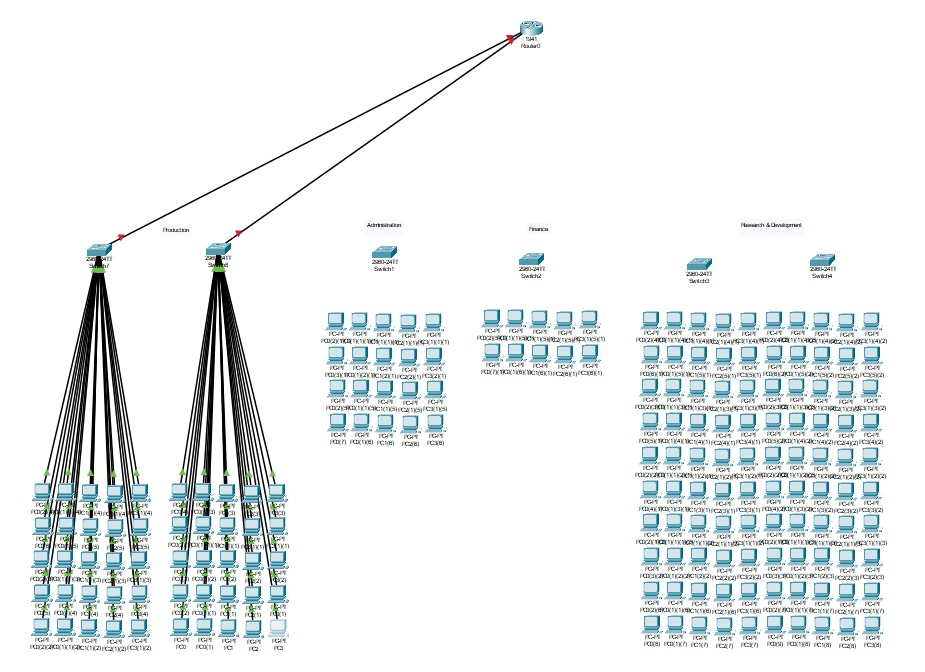
\includegraphics[width=0.5\textwidth]{P1/img/1.jpeg}
		\caption{Tampilan dalam Cisco Packet Tracer (incomplete)}
	\end{figure}
	\begin{figure}[h]
		\centering
		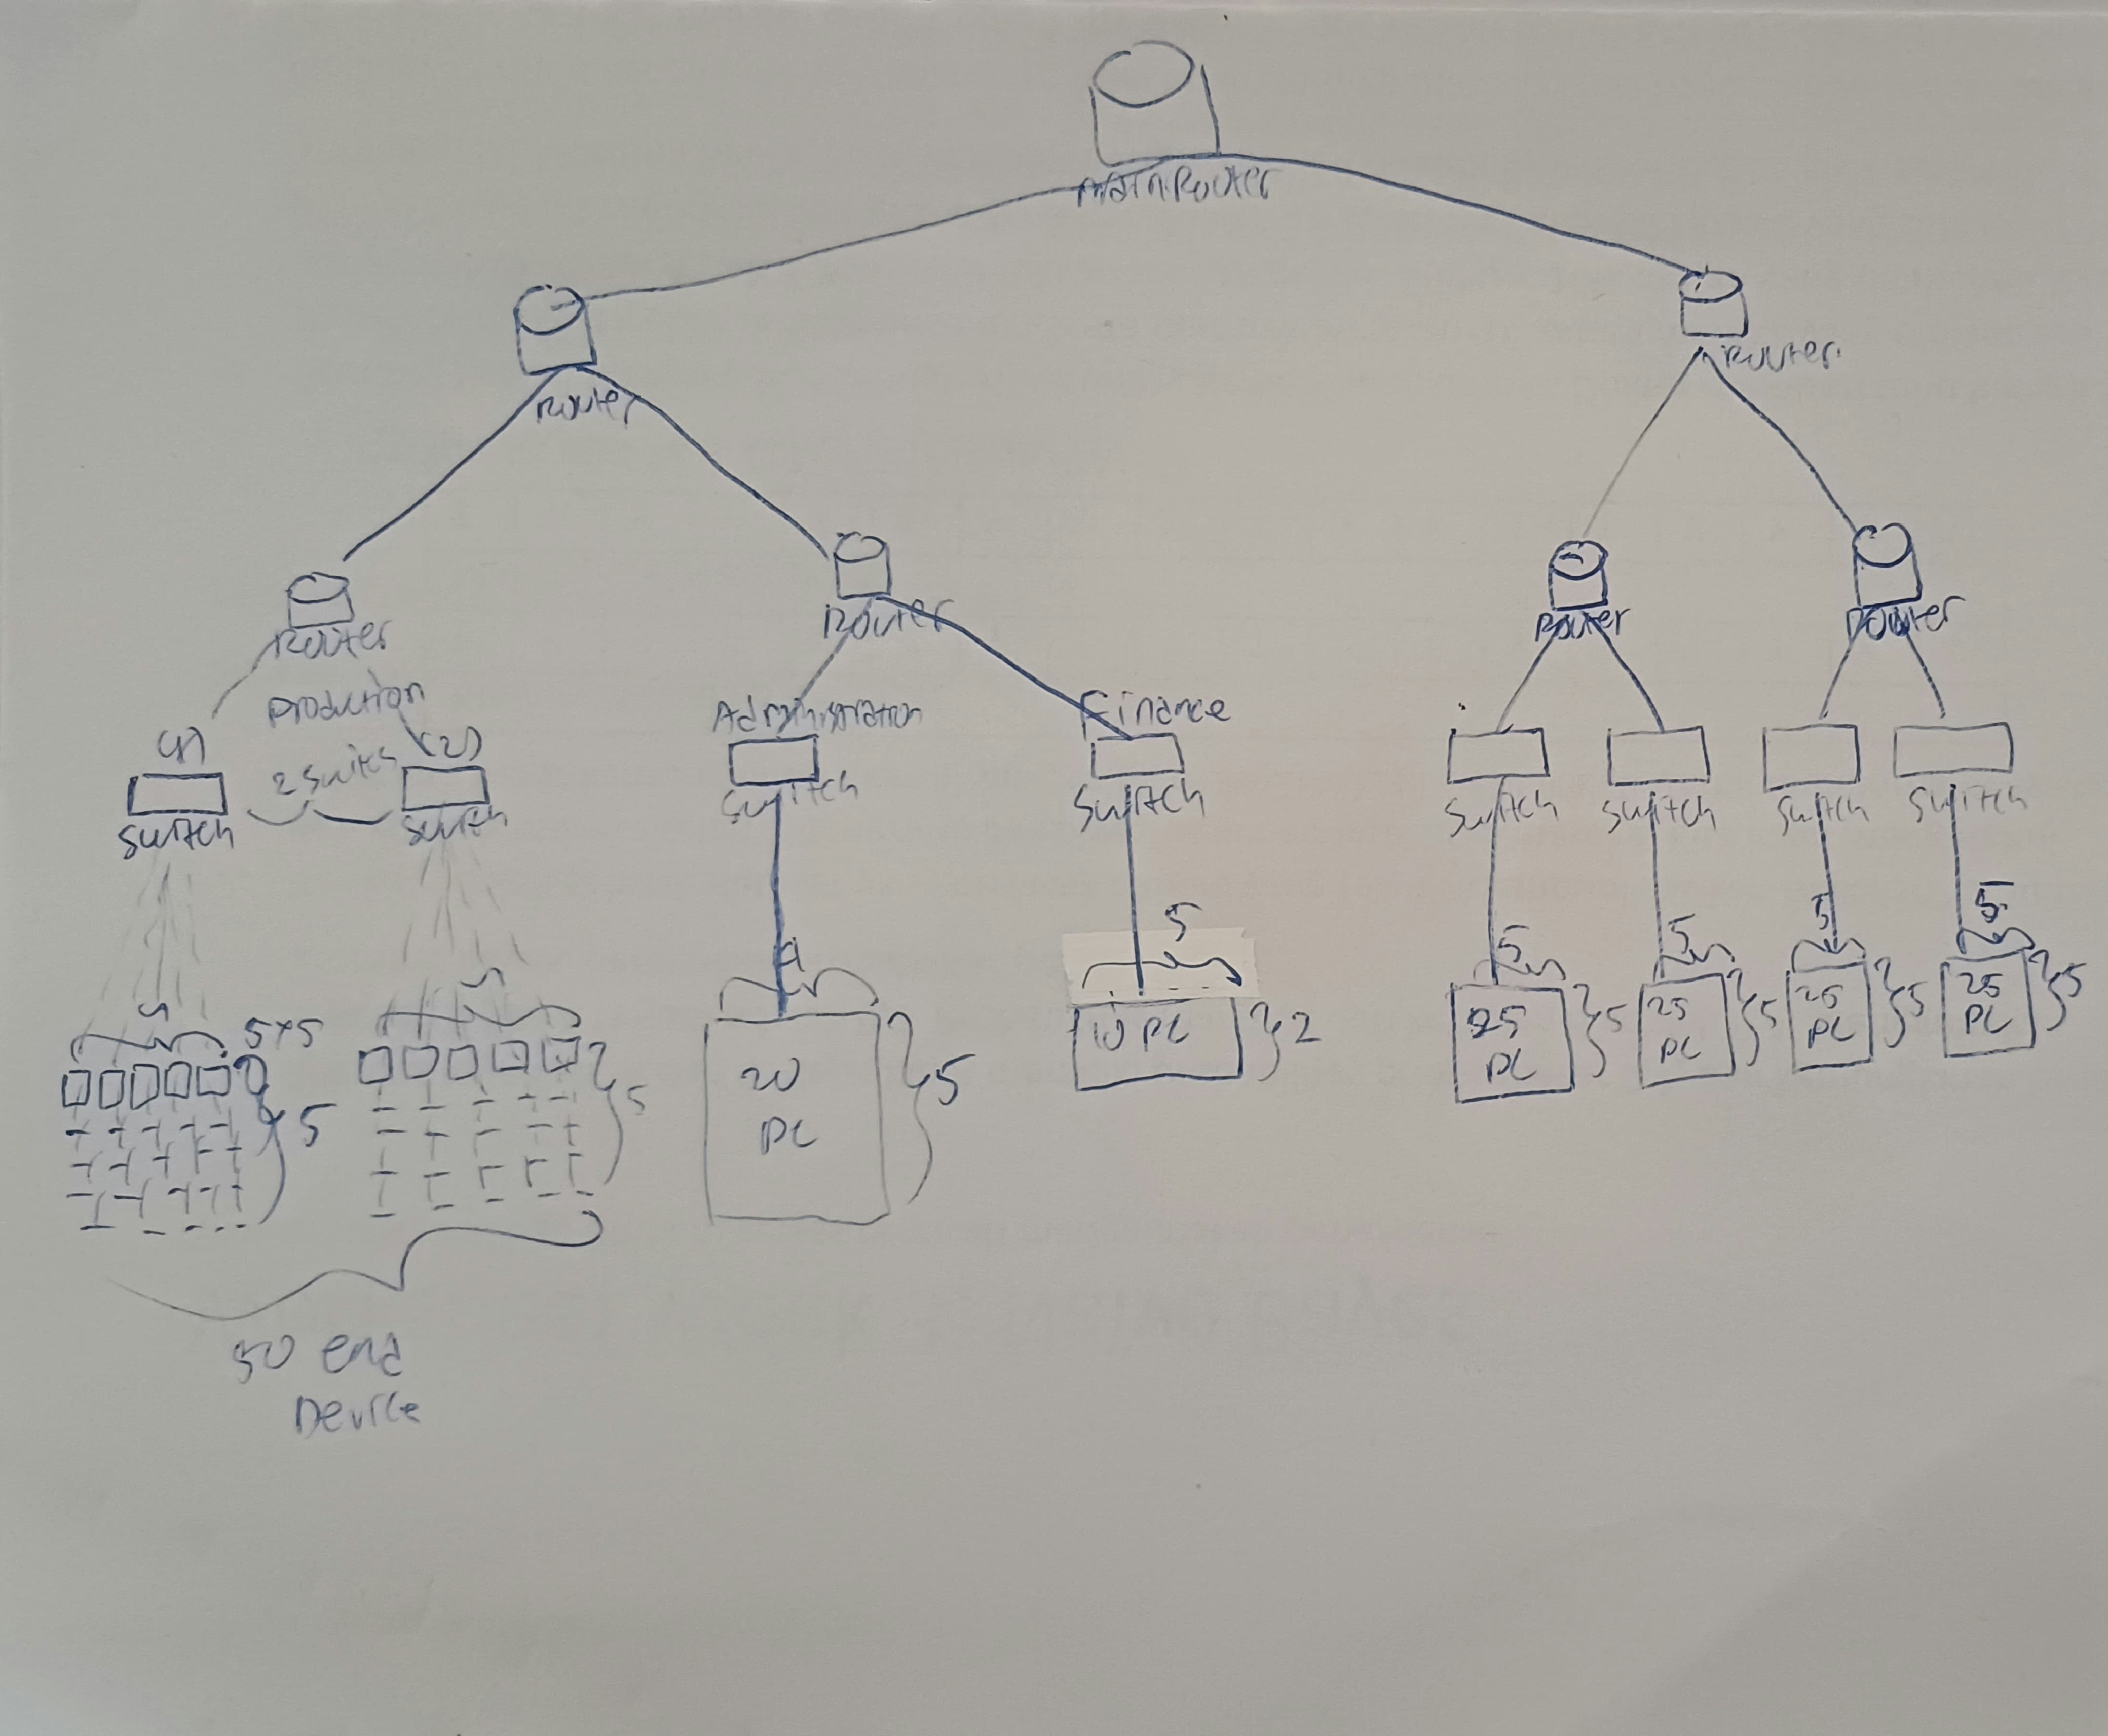
\includegraphics[width=0.5\textwidth]{P1/img/2.jpeg}
		\caption{Tampilan Topografi dalam gambar}
	\end{figure}

	\item \textbf{Tabel routing sederhana yang menunjukkan:}
	\begin{center}
		\begin{tabular}{|c|c|c|c|}
			\hline
			\textbf{Network Destination} & \textbf{Netmask/Prefix} & \textbf{Gateway} & \textbf{Interface Tujuan} \\
			\hline
			192.168.1.0 & /26 & 192.168.1.1 & eth0 \\
			192.168.1.64 & /27 & 192.168.1.1 & eth1 \\
			192.168.1.96 & /28 & 192.168.1.1 & eth2 \\
			192.168.1.128 & /25 & 192.168.1.1 & eth3 \\
			\hline
		\end{tabular}
	\end{center}
	\textbf{Penjelasan:} 
	\begin{itemize}
		\item Setiap subnet memiliki gateway yang terhubung ke interface router yang sesuai.
		\item Router bertugas untuk mengarahkan data ke subnet yang sesuai melalui interface yang tepat.
	\end{itemize}

	\item \textbf{Jenis routing yang paling cocok untuk perusahaan ini.}

	\textbf{Jenis Routing: Static Routing.}

	\textbf{Alasan:}
	\begin{itemize}
		\item Perusahaan ini memiliki jaringan dengan jumlah subnet yang relatif sedikit, yaitu empat subnet. Oleh karena itu, konfigurasi routing statis sangat efisien karena tidak memerlukan pembaruan otomatis yang terjadi pada routing dinamis.
		\item Routing statis memungkinkan administrator untuk mengontrol jalur yang akan dilalui data dengan lebih jelas, yang cocok untuk jaringan yang tidak sering berubah.
		\item Karena jaringan perusahaan ini tidak terlalu besar, routing dinamis seperti OSPF atau RIP tidak diperlukan, karena dapat menambah kompleksitas yang tidak perlu.
	\end{itemize}
\end{enumerate}
